\jxhj{%教学后记
	}
\skrq{%授课日期
	2017年12月5日 4-5节}
\ktmq{%课题名称
	 长度补偿概述}
\jxmb{%教学目标,每行前面要加 \item
	\item 掌握G43、G44、G49指令的格式;
	\item 掌握刀具相对长度的测量;
	\item 掌握刀具长度补偿的编程思路。
}
\jxzd{%教学重点,每行前面要加 \item
	\item 掌握G43、G44、G49指令的格式;
	\item 掌握刀具长度补偿的编程思路。 }
\jxnd{%教学难点,每行前面要加 \item
	\item 掌握刀具相对长度的测量。 }
\jjff{%教学方法
	通过讲述、举例、演示法来说明;}

\makeshouye %制作教案首页

%%%%教学内容
\subsection{组织教学}
\begin{enumerate}[\hspace{2em}1、]
	\item 集中学生注意力;
	\item 清查学生人数;
	\item 维持课堂纪律;
\end{enumerate}

\subsection{复习导入及主要内容}
\begin{enumerate}[1、]
\item Siemens孔加工循环概述;
\item 孔加工固定循环指令;
\item 模态调用;
\item 加工实例。
\end{enumerate}

\subsection{教学内容及过程}

加工中心或铣床在加工中都要使用很多刀具,但每把刀具的长度都不同,这样在加工时要进行长度补偿后,才能每把刀加工出来的深度都正确。

\subsubsection{补偿长度}
具安装在刀柄上,如图\ref{fig:24-1}所示,刀具安装的深度不同其补偿长度也就不同,故长度包括刀具和刀柄上的两个部分,一般就取刀具安装到主轴上后,刀具参考点到刀位点的距离,补偿长度一般就用刀具之间的相对长度。

绝对长度:刀具安装在刀柄上的整体长度,一般取刀具参考点到刀位点的距离。只用G43,无基准刀。

相对长度:待测刀相对于基准刀的长度,有正有负。

\begin{figure}[h]
	\centering
	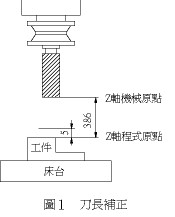
\includegraphics[width=0.7\linewidth]{data/image/24-1}
	\caption{补偿长度}
	\label{fig:24-1}
\end{figure}

\subsubsection{长度补偿方向的确定}

刀具长度补偿有G43、G44、G49三个指令:

G43为刀具长度的正补偿

G44为刀具长度的负补偿

G49为刀具取消刀具长度补偿

有两种用法:

(1)只用G43和G49指令,补偿值取正负

(2)补偿值只取正值,正负由G43及G44确定

如图\ref{fig:24-2}所示:(T1般预留)

T2设为基准刀具,相对长度为0

T3比T2短,应向Z负方向补偿,即用G44负补偿5mm;

T4比T2长,应向Z正方向补偿,即用G43正补偿7mm;

T2相对长度为0,用G49取消长度补偿。

其中,T3也可用G43正补偿-5mm。

即,只用G43和G49指令时,补偿长度的计算如下:

补偿长度=待测刀长-基准刀长 

注意:有正有负;

\begin{figure}[h]
	\centering
	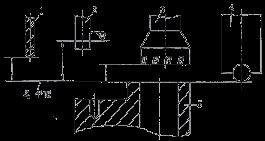
\includegraphics[width=0.7\linewidth]{data/image/24-2}
	\caption{补偿长度}
	\label{fig:24-2}
\end{figure}
\subsubsection{长度补偿值的确定}

绝对长度:刀具长度测量仪

相对长度:刀具长度测量仪

机内对刀测量法

机内自动对刀法(用G31及G10来实现)

1、用刀具长度测量仪



2、用自动对刀仪结合G31自动测量

略

3、手动的用机内对刀法测量:

A安装基准刀,将其移动到一个确定的位置,将Z向的相对坐标设置为0

B、安装待测刀,将其移动到相同的位置,记录Z向的相对坐标,这个值就是长度补偿值,有正有负。

如图\ref{fig:24-3}所示:
\begin{figure}[h]
	\centering
	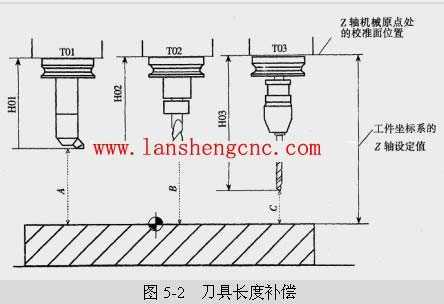
\includegraphics[width=0.7\linewidth]{data/image/24-3}
	\caption{补偿长度}
	\label{fig:24-3}
\end{figure}

\subsubsection{换刀}
数控铣床上换刀时,可在程序中加入:
\begin{lstlisting}:
G0 Z50.0
M05;
M00;
:
\end{lstlisting}
加工中心上换刀:
\begin{lstlisting}:
:
G28G91Z0;第一次换刀前要回零。

G90;
Tn M6;
G90 G1 Z100.0 G43 Hn F__;
M3 S500;
:
G0 Z____;
G49 G1 Z100.0;
M5
G0Z30.0
Tn M6
G90G43G1X
M03 S500;
\end{lstlisting}



\subsection{课堂小结}
\begin{enumerate}[1、]
\item 长度补偿概述;
\item 长度补偿方向的确定;
\item 长度补偿值的确定;
\item 换刀指令。
\end{enumerate}

\vfill
\subsection{布置作业}
\begin{enumerate}[1、]
	\item 综合习题一。
\end{enumerate}
\vfill